
\documentclass[12pt,a4paper]{article}

\usepackage[utf8]{inputenc}
\usepackage[T1]{fontenc}
\usepackage[brazil]{babel}
\usepackage{amsmath}
\usepackage{siunitx}
\usepackage{booktabs}
\usepackage{graphicx}
\usepackage[margin=2.5cm]{geometry}

\graphicspath{{figs/}}

\begin{document}

\subsection*{Caso 1}
\label{sec:res-caso1}

O \texttt{Caso 1} é o único cenário de interação fluido--estrutura (FSI) do estudo: o LCR do espaço subaracnóideo (SAS) é resolvido como fluido Newtoniano incompressível (\texttt{pimpleFluid}, OpenFOAM), acoplado bidirecionalmente à mecânica das meninges (CalculiX) pela interface \textsc{preCICE} (\texttt{fsi\_pia}, \texttt{fsi\_dura}), sob a mesma fundação de Winkler dos demais casos ($k = \SI{2e5}{\pascal\per\meter}$) e \emph{sem} a carga focal da artéria. Seu objetivo é quantificar a compartimentalização do LCR imposta pela resistência hidráulica da tampa porosa de drenagem perineural (lei de Darcy, coeficiente $d$), isolando o papel do fluido como meio transmissor de pressão à bainha. Diferente dos casos de flambagem (\texttt{C3D8I}, Neo-Hookeano), o lado sólido aqui emprega o O-grid de seção circular com núcleo neural maciço (\num{11648} hexaedros \texttt{C3D8}) e leis elásticas lineares (Tab.~\ref{tab:mat-linear}), pois a resposta é estável e sem flambagem.

A malha fluida foi verificada de forma desacoplada (\texttt{simpleFoam} laminar, $\mathrm{Re}\ll 1$), com PIC fixa de \SI{1333}{\pascal} no \emph{inlet}, referência venosa nula no \emph{outlet} e a tampa porosa no regime SANS compartimentalizado ($d = \SI{1e16}{\per\meter\squared}$), sob refino global uniforme em $r$, $\theta$ e $z$ por fator inteiro (Tabela~\ref{tab:res-caso1-malha-fluido}). A grandeza fisicamente relevante --- a pressão média no \emph{bulk} do SAS, que constitui a \emph{carga} transmitida à bainha no acoplamento --- é independente de malha até a quarta casa decimal ($\approx \SI{1333.00}{\pascal}$, variação $< \SI{0.001}{\%}$) através de uma faixa de \num{27}$\times$ no número de células (\numrange{6144}{165888}). A vazão de drenagem $Q$, indicador secundário, converge monotonicamente: a malha de produção (\num{6144} células) situa-se a $+\SI{8.1}{\%}$ da mais fina, com a variação sucessiva caindo a $\SI{2.0}{\%}$ no último refino (abaixo do critério de $\SI{5}{\%}$); a queda de pressão na tampa $\Delta p_{\mathrm{lid}}$ acompanha a mesma tendência (Figura~\ref{fig:res-caso1-malha}A). O pico local de velocidade $|U|_{\max}$ não é monotônico (extremo de malha) e por isso não é adotado como métrica de convergência, em favor das integrais robustas $p_{\mathrm{SAS}}$ e $Q$.

O O-grid estrutural foi igualmente verificado de forma desacoplada (CalculiX, elástico linear $\nu = 0.45$), substituindo o acoplamento pela carga FSI equivalente (pressão estática $p_{\mathrm{SAS}} = \SI{3800}{\pascal}$ nas faces \texttt{fsi\_pia}/\texttt{fsi\_dura}), sob refino global do O-grid por fator inteiro (Tabela~\ref{tab:res-caso1-malha-solido}). A QoI física do caso --- a distensão radial máxima da dura $\Delta r_{\mathrm{dura}}$, achado clínico da SANS --- converge monotonicamente, com a malha de produção (\num{11648} elementos) já a apenas $\SI{1.06}{\%}$ da malha mais fina (\num{314496} elementos) e variações sucessivas $< \SI{0.6}{\%}$ (Figura~\ref{fig:res-caso1-malha}B). Por ser uma resposta linear-elástica e estável (sem flambagem), o caso dispensa o estudo local/modal exigido pelos cenários de instabilidade (Casos~2 e~3); o pico de von Mises, concentrado no engaste e de natureza local, converge mais lentamente e é reportado apenas como indicador, em favor da métrica integral $\Delta r_{\mathrm{dura}}$.

\begin{table}[h!]
\centering
\small
\caption{Caso 1, independência de malha do lado fluido (\texttt{simpleFoam}, carga SANS fixa: PIC \SI{1333}{\pascal} no \emph{inlet}, tampa Darcy $d = \SI{1e16}{\per\meter\squared}$). $p_{\mathrm{SAS}}$ é a pressão média no \emph{bulk} (carga transmitida à bainha); $Q$ a vazão de drenagem distal; $\Delta p_{\mathrm{lid}}$ a queda na tampa porosa. A coluna $\Delta Q$ é a variação sucessiva entre níveis.}
\label{tab:res-caso1-malha-fluido}
\begin{tabular}{l r r r r r}
\toprule
\textbf{Nível} & \textbf{nCélulas} & $p_{\mathrm{SAS}}$ (\si{\pascal}) & $Q$ (\si{\meter\cubed\per\second}) & $\Delta p_{\mathrm{lid}}$ (\si{\pascal}) & $\Delta Q$ (\si{\%}) \\
\midrule
produção (\texttt{x1}) & 6144   & 1332.9999 & $2.941\times10^{-12}$ & 522.9 & ---  \\
\texttt{x2}            & 49152  & 1332.9999 & $2.777\times10^{-12}$ & 607.2 & 5.9  \\
\texttt{x3}            & 165888 & 1332.9999 & $2.721\times10^{-12}$ & 631.2 & 2.0  \\
\bottomrule
\end{tabular}
\end{table}

\begin{table}[h!]
\centering
\small
\caption{Caso 1, independência de malha do lado sólido (O-grid, CalculiX elástico linear, carga FSI equivalente $p_{\mathrm{SAS}} = \SI{3800}{\pascal}$). $\Delta r_{\mathrm{dura}}$ é a distensão radial máxima da bainha (QoI física); $\Delta r_{\mathrm{pia}}$ a da pia; $\sigma_{vM}$ o pico global de von Mises. A coluna $\Delta(\Delta r_{\mathrm{dura}})$ é a variação sucessiva entre níveis.}
\label{tab:res-caso1-malha-solido}
\begin{tabular}{l r r r r r}
\toprule
\textbf{Nível} & \textbf{nElem.} & $\Delta r_{\mathrm{dura}}$ (\si{\micro\meter}) & $\Delta r_{\mathrm{pia}}$ (\si{\micro\meter}) & $\sigma_{vM}$ (\si{\kilo\pascal}) & $\Delta(\Delta r_{\mathrm{dura}})$ (\si{\%}) \\
\midrule
produção (\texttt{f1}) & 11648  & 42.84 & 19.70 & 58.45 & ---  \\
\texttt{f2}            & 93184  & 42.64 & 19.19 & 58.01 & 0.46 \\
\texttt{f3}            & 314496 & 42.39 & 18.95 & 57.98 & 0.60 \\
\bottomrule
\end{tabular}
\end{table}

\begin{figure}[h!]
\centering
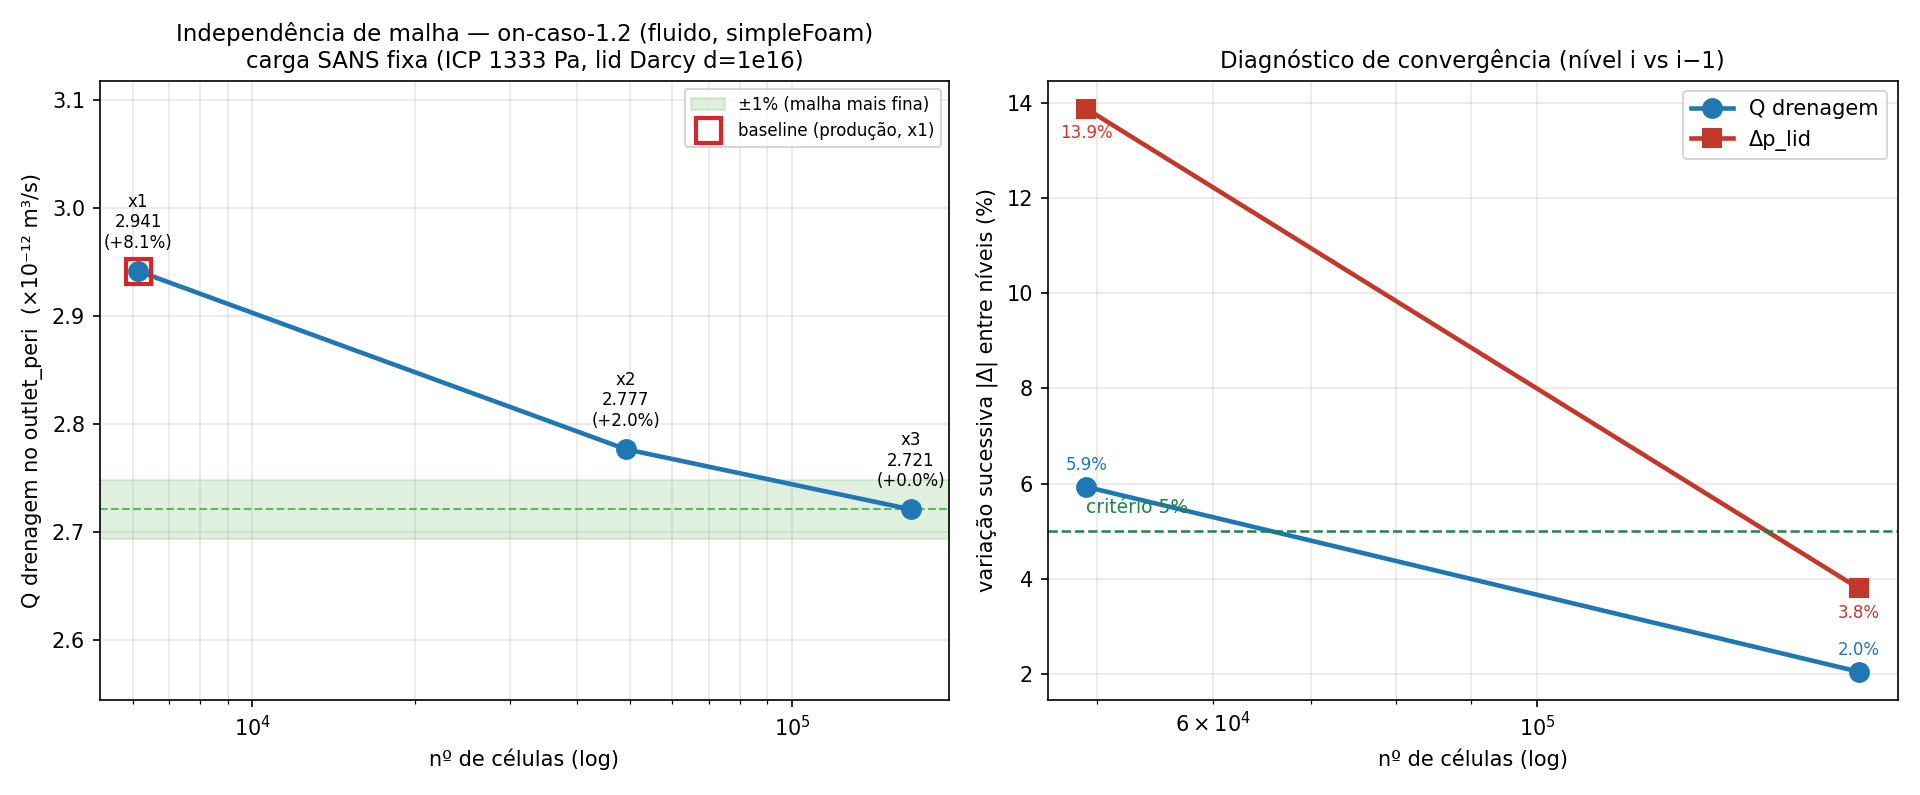
\includegraphics[width=0.49\linewidth]{on-caso-1.2-mesh-independence-fluid.png}
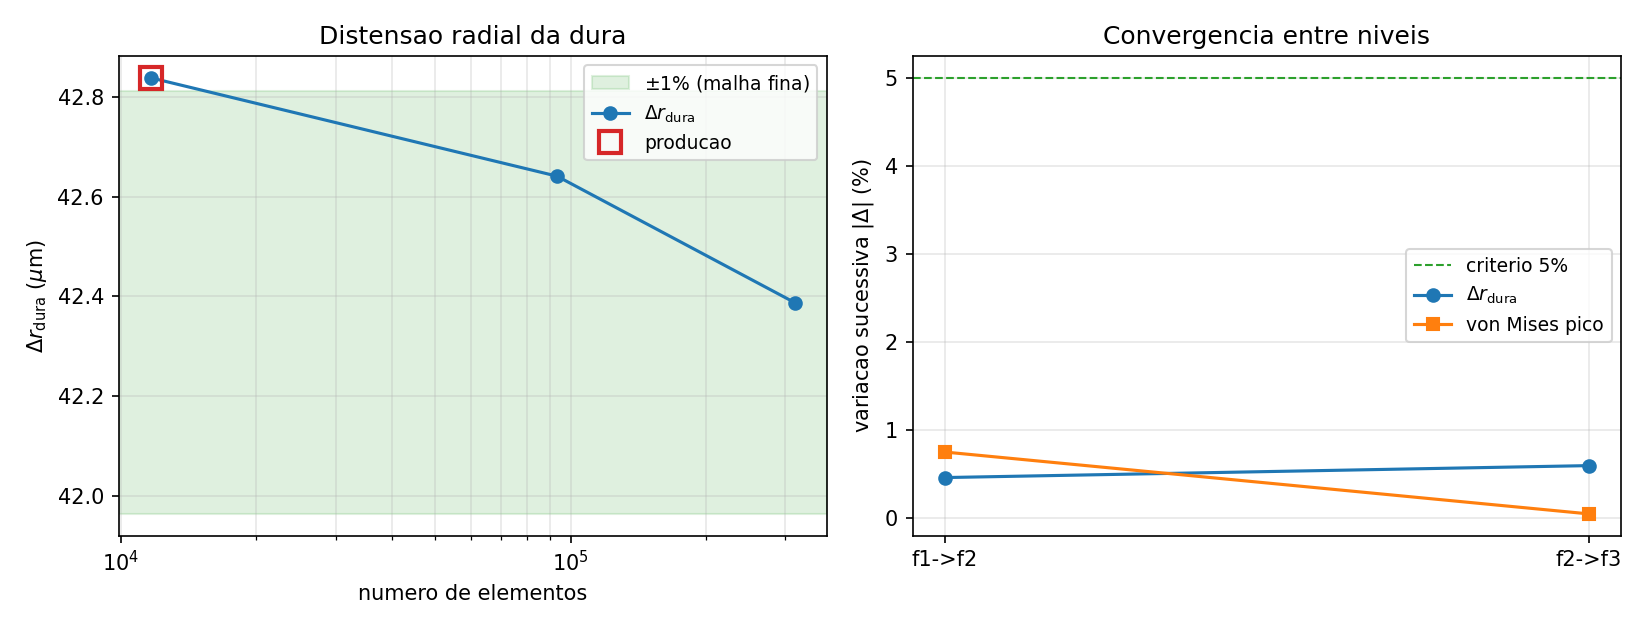
\includegraphics[width=0.49\linewidth]{on-caso-1.2-mesh-independence-solid.png}
\caption{Caso 1, independência de malha desacoplada. (A)~Lado fluido: vazão de drenagem $Q$ vs número de células (escala log) com faixa de $\pm\SI{1}{\%}$ em torno da malha mais fina; a malha de produção (marcador vermelho) já situa-se próxima da convergência e a variação sucessiva cai abaixo do critério de $\SI{5}{\%}$. (B)~Lado sólido: distensão radial da dura $\Delta r_{\mathrm{dura}}$ vs número de elementos; a malha de produção fica a $\SI{1.06}{\%}$ da mais fina, dentro da faixa de $\pm\SI{1}{\%}$.}
\label{fig:res-caso1-malha}
\end{figure}

Com a PIC fixa no \emph{inlet} e a saída perineural livre, a varredura $d \in \{10^{13};\,10^{15};\,10^{17}\}\,\si{\per\meter\squared}$ reproduz escalamento de Darcy puro: a vazão de drenagem $Q$ cai de \SI{9.96e-10}{} (tampa aberta) a \SI{9.96e-14}{\meter\cubed\per\second} (compartimentalização tipo IIH/SANS), passando pelo regime fisiológico saudável $\sim\SI{1e-11}{\meter\cubed\per\second}$ em $d = \SI{1e15}{\per\meter\squared}$ --- uma queda de $100\times$ por década de $d$ (Figura~\ref{fig:res-caso1-comp}). Como as pressões de contorno estão ancoradas, a compartimentalização manifesta-se no \emph{fluxo}, mapeando diretamente o grau de obstrução das vilosidades aracnoides perineurais que drenam o LCR do ONSAS.

\begin{figure}[h!]
\centering
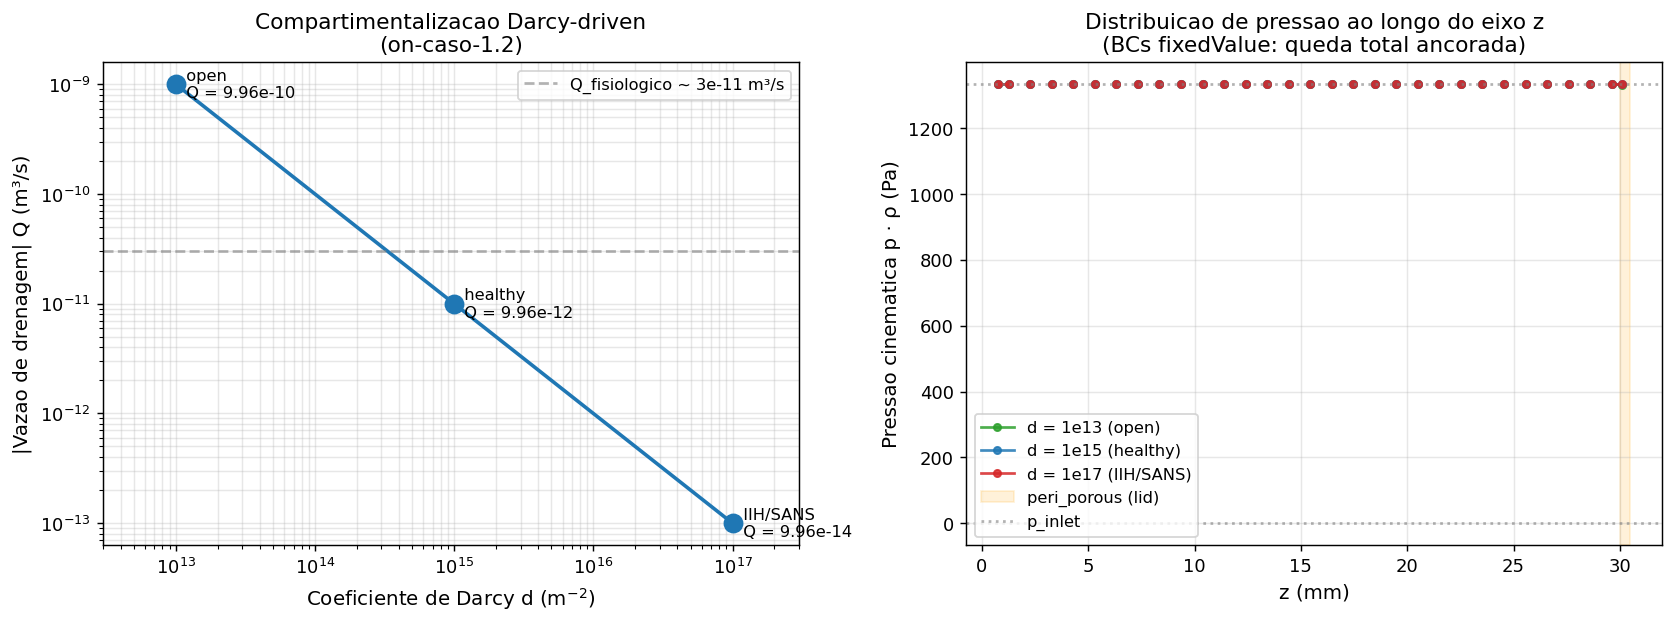
\includegraphics[width=0.85\linewidth]{on-caso-1.2-compartmentalization.png}
\caption{Caso 1 (FSI, modo de pressão prescrita). À esquerda, vazão de drenagem $Q$ vs coeficiente de Darcy $d$ (escala log--log): escalamento de Darcy puro, com $Q$ caindo $100\times$ por década, do regime aberto (\SI{9.96e-10}{\meter\cubed\per\second}) ao compartimentalizado IIH/SANS (\SI{9.96e-14}{\meter\cubed\per\second}), passando pelo fisiológico ($\sim\SI{1e-11}{\meter\cubed\per\second}$). À direita, perfil de pressão $p(z)$: com as pressões de contorno ancoradas, a compartimentalização manifesta-se no fluxo, não na pressão do \emph{bulk}.}
\label{fig:res-caso1-comp}
\end{figure}

Substituindo o \emph{inlet} de pressão por uma vazão fisiológica fixa ($Q_{\mathrm{in}} = \SI{3e-11}{\meter\cubed\per\second}$), qualquer aumento de $d$ obriga a uma elevação proporcional da pressão no \emph{bulk} do SAS --- exatamente a hipótese fisiopatológica da SANS. A PIC no \emph{bulk} transita de regime aberto (valores negativos, dominados por Bernoulli transiente) para o saudável ($\approx \SI{1106}{\pascal}$, da ordem da PIC basal de \SI{1333}{\pascal}) em $d = \SI{1e15}{\per\meter\squared}$, e salta para $\approx \SI{14039}{\pascal}$ ($\sim\SI{105}{mmHg}$, hipertensão intracraniana severa) em $d = \SI{1e16}{\per\meter\squared}$ (Tabela~\ref{tab:res-caso1-pic}). A transição de saudável a severo concentra-se numa \emph{única} década de $d$ (fator $12.7\times$ na PIC), reproduzindo a observação clínica de que pequenas variações na permeabilidade das vias de drenagem disparam de forma abrupta a compartimentalização do ONSAS.

\begin{table}[h!]
\centering
\small
\caption{Caso 1, modo dirigido pela PIC (vazão prescrita $Q_{\mathrm{in}} = \SI{3e-11}{\meter\cubed\per\second}$). PIC no \emph{bulk} do SAS e queda de pressão na tampa porosa $\Delta p_{\mathrm{lid}}$ em função do coeficiente de Darcy $d$. A transição de saudável a severo ocorre numa única década de $d$.}
\label{tab:res-caso1-pic}
\begin{tabular}{r r r l}
\toprule
$d$ (\si{\per\meter\squared}) & $\mathrm{PIC}_{\mathrm{bulk}}$ (\si{\pascal}) & $\Delta p_{\mathrm{lid}}$ (\si{\pascal}) & Regime \\
\midrule
$10^{12}$ & $-330$  & $-85$  & tampa aberta (Bernoulli) \\
$10^{13}$ & $-317$  & $-81$  & idem \\
$10^{14}$ & $-188$  & $-36$  & quase aberto \\
$10^{15}$ & $1106$  & $410$  & \textbf{saudável} ($\sim$PIC basal) \\
$10^{16}$ & $14039$ & $4871$ & \textbf{IIH/SANS severo} ($\sim$\SI{105}{mmHg}) \\
\bottomrule
\end{tabular}
\end{table}

\begin{figure}[h!]
\centering
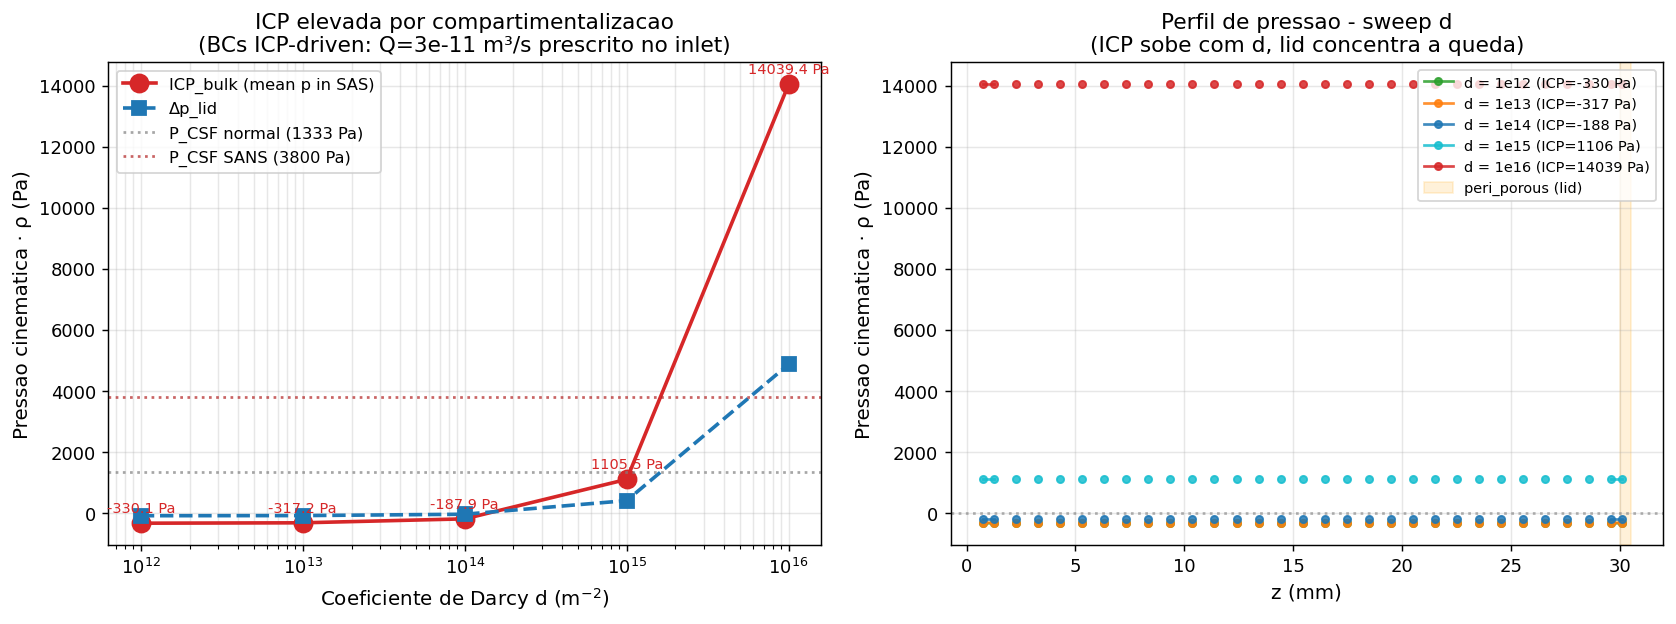
\includegraphics[width=0.85\linewidth]{on-caso-1.2-pic-driven.png}
\caption{Caso 1 (FSI, modo dirigido pela PIC). À esquerda, PIC no \emph{bulk} do SAS e queda na tampa $\Delta p_{\mathrm{lid}}$ em função do coeficiente de Darcy $d$; a transição de saudável (\SI{1333}{\pascal}) a SANS severo ($\sim\SI{14}{\kilo\pascal}$) ocorre numa única década de $d$. À direita, perfil de pressão $p(z)$ ao longo do eixo do nervo: a PIC sobe uniformemente no \emph{bulk} e a queda concentra-se na tampa porosa distal.}
\label{fig:res-caso1-pic}
\end{figure}

No acoplamento bidirecional completo, com a PIC prescrita em rampa de \SI{1333}{} a \SI{3800}{\pascal} (saudável $\to$ SANS) ao longo de seis janelas, o LCR pressurizado transmite a carga simultaneamente às duas interfaces: a dura \emph{expande} radialmente para fora ($+\SI{0.439}{\micro\meter}$ líquidos no \emph{watchpoint} peripapilar $z = \SI{30}{\milli\meter}$, $\theta = 0$) enquanto a pia é \emph{comprimida} para dentro ($-\SI{0.370}{\micro\meter}$), estreitando o espaço perineural por ambos os lados (Figura~\ref{fig:res-caso1-dura}). Essa resposta de sinal oposto nas duas paredes é a assinatura mecânica do princípio de Pascal num compartimento fechado de baixa complacência: o fluido recupera a pressão isotrópica que um SAS modelado como sólido hidrostático equivalente (Casos~2 e~3) não captura, distendendo a bainha (achado de imagem da SANS) ao mesmo tempo que aperta o nervo. A distensão radial máxima da dura sob a carga plena equivalente atinge $\approx \SI{42.8}{\micro\meter}$ na verificação desacoplada (Tabela~\ref{tab:res-caso1-malha-solido}), confirmando a magnitude da distensão da bainha como grandeza convergida e independente de malha.

\begin{figure}[h!]
\centering
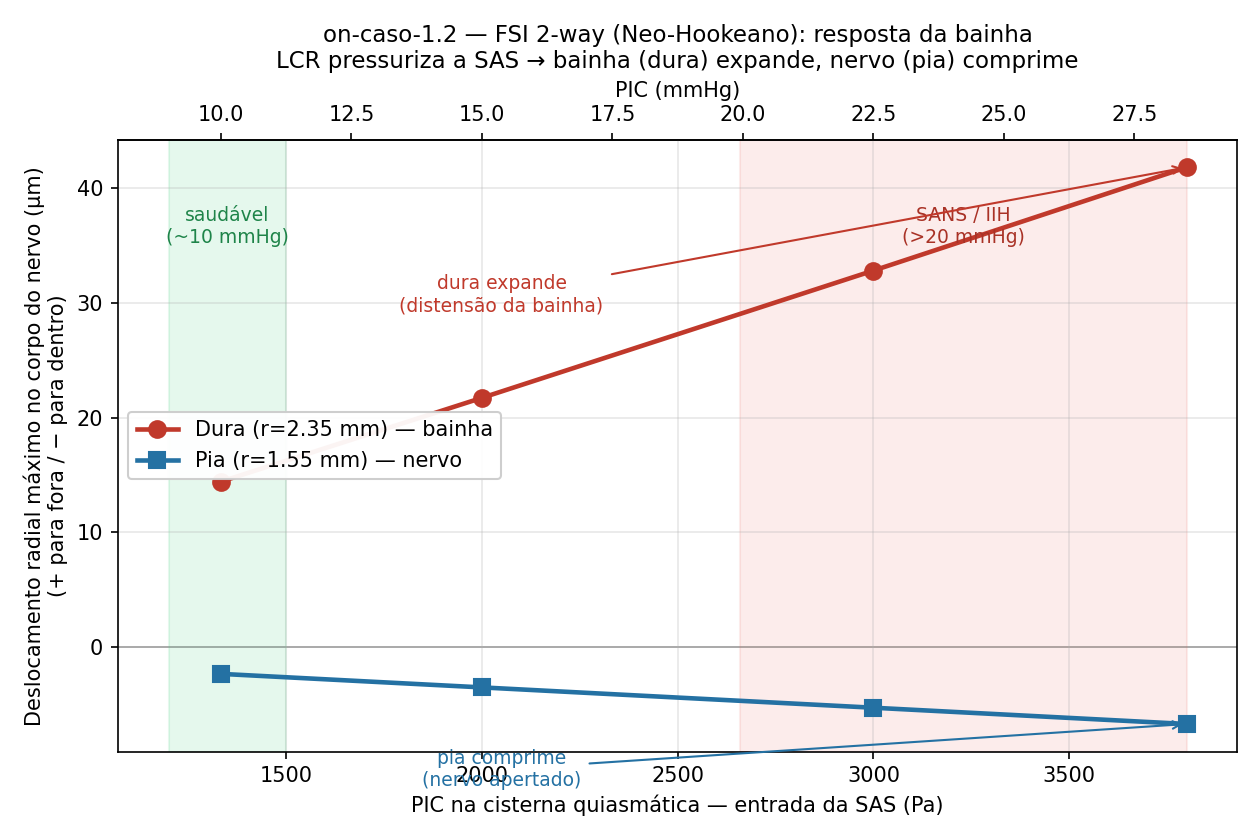
\includegraphics[width=0.8\linewidth]{on-caso-1.2-dura-expansion.png}
\caption{Caso 1 (FSI 2-way). Deslocamento radial no \emph{watchpoint} peripapilar ($z = \SI{30}{\milli\meter}$, $\theta = 0$) sob a rampa de PIC de \SI{1333}{} (saudável) a \SI{3800}{\pascal} (SANS/IIH). A dura (bainha) expande monotonicamente para fora e a pia (nervo) é comprimida para dentro: o LCR pressurizado, ao recuperar a pressão isotrópica de Pascal, distende a bainha e estrangula o nervo simultaneamente.}
\label{fig:res-caso1-dura}
\end{figure}

O acoplamento FSI completo no modo dirigido pela PIC com material Neo-Hookeano diverge para $\mathrm{PIC}_{\mathrm{bulk}} > \SI{1500}{\pascal}$ ($d \ge \SI{1e15}{\per\meter\squared}$), por falha do método de Newton--Raphson do CalculiX: as forças FSI excedem a capacidade portante das lâminas pia e dura no regime hiperelástico. O regime severo da Tabela~\ref{tab:res-caso1-pic} foi, portanto, obtido no caso auxiliar \emph{fluid-only} (\texttt{on-caso-1.2-fluidonly}, mesma malha e \texttt{fvOptions}, sem o lado estrutural). A extensão ao acoplamento completo sob PIC elevada requer \emph{ramping} de carga em múltiplos passos ou amortecimento, e fica como trabalho futuro.

\end{document}
